% ===========================================================================
\section{O desenho do crivo}\label{sec:desenho}
% ===========================================================================

Temos um dicionário (Seção~\ref{sec:dicionario}) e uma base canônica para cada
bloco (Seção~\ref{sec:blocos}). Falta o instrumento que torna o dicionário
visível. Ele vem, sem surpresa, do fator de Euler.

\subsection{O tom de um inteiro}

Seja $s=\tfrac12+it$ com $t\in\R$. Para $m\ge2$,
\[
  \bigl|1-m^{-s}\bigr|^2
  \;=\; 1-2\,m^{-1/2}\cos\bigl(t\nfreq m\bigr)+m^{-1},
\]
de modo que o logaritmo do módulo do fator de Euler correspondente é
\begin{equation}\label{eq:Sm}
  S_m(t) \;=\; -\tfrac12\log\!\Bigl(1-2\,m^{-1/2}\cos\bigl(t\nfreq m\bigr)+m^{-1}\Bigr).
\end{equation}

\begin{lema}[série de Fourier de $S_m$]\label{lema:serie}
Para todo $t\in\R$,
\begin{equation}\label{eq:serie}
  S_m(t) \;=\; \sum_{k\ge1}\frac{m^{-k/2}}{k}\,\cos\bigl(k\,t\,\nfreq m\bigr).
\end{equation}
Em particular $S_m$ é limitada e positiva, e sua componente fundamental oscila
com frequência $\freq m=\nfreq m/2\pi$ e amplitude $m^{-1/2}$.
\end{lema}

\begin{proof}
Com $a=m^{-1/2}\in(0,1)$ e $\theta=t\nfreq m$, a identidade clássica
$\log(1-2a\cos\theta+a^2)=-2\sum_{k\ge1}\frac{a^k}{k}\cos(k\theta)$ — que segue da
série de $\log(1-z)$ em $|z|<1$, tomando $z=ae^{i\theta}$ e $z=ae^{-i\theta}$ e
somando — dá \eqref{eq:serie} após multiplicar por $-\tfrac12$.
\end{proof}

A série \eqref{eq:serie} é a tradução sonora do dicionário. O inteiro $m$ emite um
tom fundamental na sua frequência e harmônicos nos múltiplos inteiros dessa
frequência, com amplitudes que decaem geometricamente. Um composto emite, por
construção, um tom fundamental que é a \emph{soma} das frequências dos seus
fatores — o que o Lema~\ref{lema:homomorfismo} garante — e cujos harmônicos também
coincidem com combinações das frequências dos fatores.

\subsection{Ortogonalidade}

\begin{lema}[ortogonalidade]\label{lema:orto}
Sejam $\alpha,\beta>0$ e $T>0$. Então
\[
  \frac1T\int_0^T\cos(\alpha t)\cos(\beta t)\,dt
  =
  \begin{cases}
    \dfrac12+O\!\left(\dfrac{1}{T\alpha}\right), & \alpha=\beta,\\[10pt]
    O\!\left(\dfrac{1}{T|\alpha-\beta|}\right), & \alpha\neq\beta .
  \end{cases}
\]
\end{lema}

\begin{proof}
A identidade de produto de cossenos reduz a integral a
$\tfrac12\int_0^T\cos((\alpha-\beta)t)\,dt+\tfrac12\int_0^T\cos((\alpha+\beta)t)\,dt$,
e $\bigl|\int_0^T\cos(\gamma t)\,dt\bigr|\le 2/|\gamma|$ para $\gamma\neq0$,
enquanto $\int_0^T1\,dt=T$.
\end{proof}

O Lema~\ref{lema:orto} é o que autoriza ler amplitudes: sobre uma janela longa, o
coeficiente de um sinal em uma frequência é determinado — a menos de $O(1/T)$ —
pela componente que oscila exatamente naquela frequência. As frequências
$\nfreq m$ de inteiros distintos nunca coincidem, porque $\nfreq{}$ é injetora.

\subsection{O resíduo de um bloco}

Seja $I$ um conjunto finito de inteiros e defina
\[
  Z_I(t) \;=\; \sum_{m\in I} S_m(t).
\]
Para $p$ primo com $n=\lfloor\log_2 p\rfloor$, tome o intervalo
$I_p=[2^{n-1},p-1]$ e separe-o em primos e compostos:
$I_p = \Pi \sqcup C$, com $\Pi=\{q\in I_p: q \text{ primo}\}$ e $C$ o resto. Então
\begin{equation}\label{eq:residuo}
  R(t) \;=\; Z_{I_p}(t)-Z_C(t) \;=\; Z_{\Pi}(t) \;=\; \sum_{q\in\Pi} S_q(t).
\end{equation}

A identidade \eqref{eq:residuo} é exata, para todo $t$, por linearidade da soma:
subtrair o sinal dos compostos remove exatamente esses termos e não toca nos
demais. Não há aproximação envolvida \emph{na construção}. O que há é uma escolha
de representação: em vez de olhar $Z_{I_p}$, olhamos o resíduo, que contém apenas
os tons dos primos do bloco.

A Figura~\ref{fig:desenho} mostra o resultado para $p=37$, isto é,
$I_p=[16,36]$. À esquerda, o espectro de $Z_{I_p}$: vinte e uma oscilações
superpostas, sem estrutura legível. À direita, o espectro de $R$: cinco picos
isolados, e eles estão exatamente nas frequências dos cinco primos do intervalo —
$17,19,23,29,31$.

\begin{figure}[htbp]
\centering
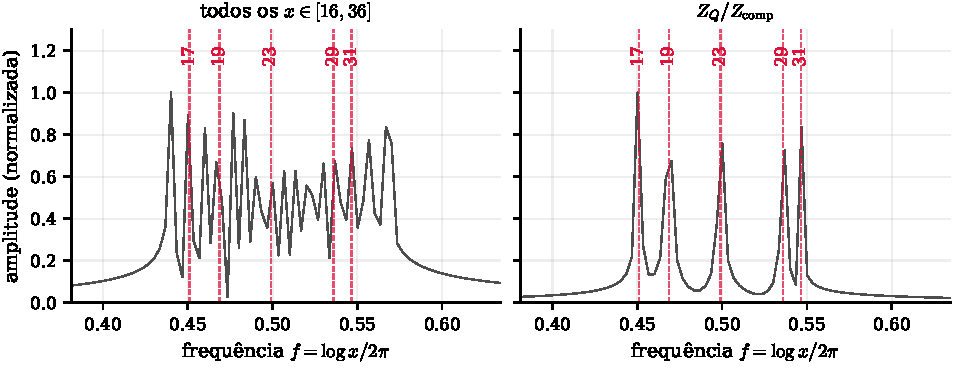
\includegraphics[width=0.98\textwidth]{figuras/f1_desenho.pdf}
\caption{O bloco $I_p=[16,36]$ de $Q(37)$, com $t_{\max}=300$ e passo
$\Delta t=0{,}02$. À esquerda, o espectro de $Z_{I_p}$, que soma os vinte e um
inteiros do intervalo. À direita, o resíduo \eqref{eq:residuo}, obtido subtraindo
o sinal dos compostos: restam os tons dos cinco primos, nas posições previstas
pelo dicionário.}
\label{fig:desenho}
\end{figure}

Vale registrar o que a figura \emph{não} faz. Ela não decide primalidade: a
subtração em \eqref{eq:residuo} usa a lista $\Pi$, isto é, usa a informação
aritmética que se quer representar. O que a figura oferece é uma
\emph{representação} dessa informação — uma em que cada primo é um objeto visual
distinguível, com posição e altura determinadas pela sua frequência e pelo seu
tamanho.

\subsection{A outra metade do reticulado}

O resíduo \eqref{eq:residuo} contém os primos do intervalo $I_p$, isto é, os
primos entre $2^{n-1}$ e $p$. Os primos menores — a semente $\Seed_{n}$ — não
estão lá como tons diretos. Eles aparecem, porém, de outra forma: como
\emph{divisores} dos compostos de $I_p$, e portanto como frequências presentes no
sinal dos compostos que acabamos de subtrair.

Há uma maneira clássica de extrair essa contribuição: comparar $Z_{I_p}$ com a
função zeta, cujo produto de Euler percorre todos os primos \cite{titchmarsh}. A
diferença
\[
  Z_{I_p}(t)-\log\bigl|\zeta(\tfrac12+it)\bigr|
\]
cancela os primos do intervalo, que aparecem nos dois lados, e deixa visíveis os
primos pequenos, que no intervalo aparecem apenas através de múltiplos. O preço é
ter de avaliar $\zeta$ na linha crítica em precisão suficiente, o que é caro; e a
alternativa aritmética da Seção~\ref{sec:blocos} obtém a semente por recursão, sem
números complexos.

Mencionamos o artifício porque ele fecha a imagem: o dicionário comporta as duas
metades do reticulado, os primos do bloco como tons diretos e a semente como
ressonância nos compostos. A Figura~\ref{fig:desenho} mostra a primeira metade; a
segunda é mais difícil de ver e não a usaremos adiante.

\subsection{Quanta resolução é necessária}

Um pico é um objeto de largura finita. A janela de observação $[0,T]$ dá à
transformada uma resolução em frequência da ordem de $1/T$ (Lema~\ref{lema:orto}),
e dois primos consecutivos $q_1<q_2$ só aparecem como picos separados se
\[
  \frac{1}{T} \;\ll\; \freq{q_2}-\freq{q_1}
  \;=\; \frac{\log(q_2/q_1)}{2\pi} .
\]
Isso é o conteúdo da próxima seção, onde a desigualdade é tornada exata e o custo
do desenho é calculado. A Figura~\ref{fig:resolucao} antecipa o efeito: o mesmo
bloco de $Q(53)$, desenhado com duas janelas diferentes, revela ou esconde os
pares mais próximos.

\begin{figure}[htbp]
\centering
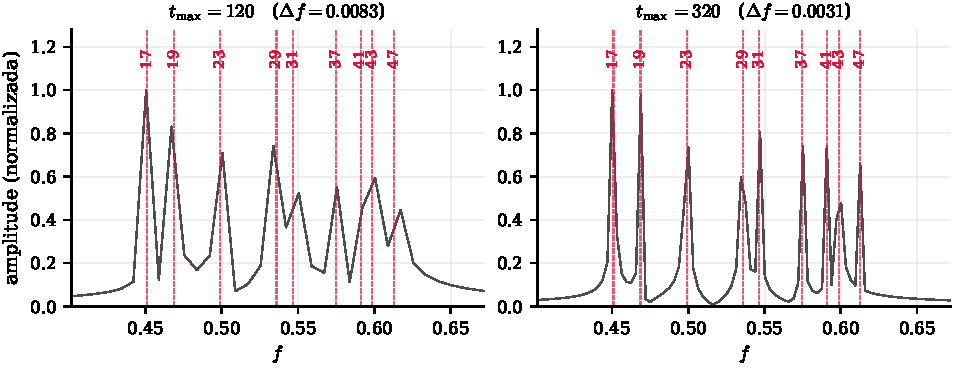
\includegraphics[width=0.98\textwidth]{figuras/f2_resolucao.pdf}
\caption{O bloco $I_p=[32,52]$ de $Q(53)$ com duas janelas. À esquerda,
$t_{\max}=120$: os pares de primos consecutivos mais próximos aparecem fundidos,
e o desenho conta menos picos do que primos. À direita, $t_{\max}=320$: todos os
primos do bloco são resolvidos. A posição dos picos é a mesma nos dois casos; o
que muda é a capacidade de separá-los.}
\label{fig:resolucao}
\end{figure}
